\documentclass{standalone}
\usepackage{amsmath,amssymb,amsthm}
\usepackage[usenames,dvipsnames,table]{xcolor}
%\usepackage{graphicx} 										% Graphics
\usepackage{tikz} \usetikzlibrary{calc,arrows.meta,positioning, intersections, patterns} 	% Figure

	\definecolor{MyGreen}{rgb}{0.33, 0.42, 0.18}
	\definecolor{MyRed}{rgb}{0.6, 0.1, 0.1}
	\definecolor{MyTurquoise}{rgb}{0.20, 0.50, 0.52}
	\definecolor{MyBlue}{rgb}{0, 0.25, 0.5}
	\definecolor{MyOldViolet}{rgb}{0.44, 0.16, 0.39}
	\definecolor{MyYellow}{rgb}{1, 0.65, 0}

	%Colored
%	\tikzstyle{arrow} =  	      [->,outer sep=14pt, draw=black, text = black]
%	\tikzstyle{enterexit} =      [rectangle, minimum height=0cm, text width=1.5cm, text = black, draw=none]
%	% Full color
%	\tikzstyle{vaccinated} =    [rectangle, minimum height=1cm, text width=1.5cm, text = white, fill=MyBlue]
%	\tikzstyle{susceptible} =  [rectangle, minimum height=1cm, text width=1.5cm, text = white, fill=MyOldViolet]
%	\tikzstyle{exposed} =  [rectangle, minimum height=1cm, text width=1.5cm, text = white, fill=MyYellow]
%	\tikzstyle{infectious} =     [rectangle, minimum height=1cm, text width=1.5cm, text = white, fill=MyRed]
%	\tikzstyle{recovered} =    [rectangle, minimum height=1cm, text width=1.5cm, text = white, fill=MyGreen]
%	\tikzstyle{treated} = 	      [rectangle, minimum height=1cm, text width=1.5cm, text = white, fill=MyTurquoise]
	
	% B&W
	\tikzstyle{arrow} = [->,outer sep=14pt, draw=black, text = black]
	\tikzstyle{enterexit} = [rectangle, minimum height=0cm, text width=1.5cm, text = black, draw=none]
	% Full color
	\tikzstyle{vaccinated} = [rectangle, minimum height=1cm, text width=1.5cm, text = white, fill=black]
	\tikzstyle{susceptible} = [rectangle, minimum height=1cm, text width=1.5cm, text = black, fill=black!20]
	\tikzstyle{exposed} = [rectangle, minimum height=1cm, text width=1.5cm, text = black, fill=black!20]
	\tikzstyle{infectious} = [rectangle, minimum height=1cm, text width=1.5cm, text = black, fill=black!20]
	\tikzstyle{recovered} = [rectangle, minimum height=1cm, text width=1.5cm, text = black, fill=black!20]
	\tikzstyle{treated} = [rectangle, minimum height=1cm, text width=1.5cm, text = black, fill=black!20]


\begin{document}
	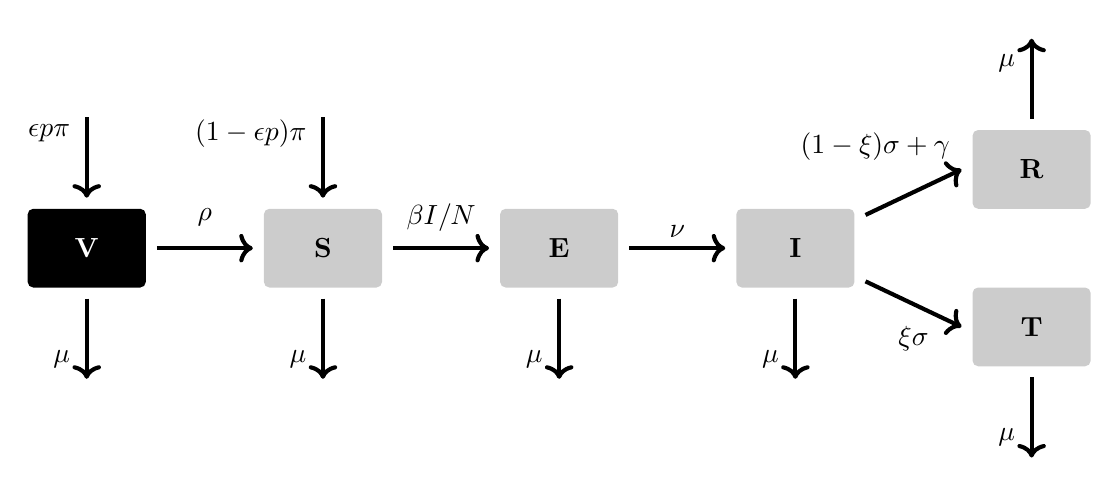
\begin{tikzpicture}[node distance=4cm,text centered,rounded corners=2pt, outer sep=4pt,inner sep=0pt,line width=1.5pt]
		\node (V) [vaccinated] 					{{\bf V}};
		\node (S) [right of=V,xshift=-1cm,susceptible] 			{{\bf S}};
		\node (E) [right of=S,xshift=-1cm,exposed] 				{{\bf E}};
		\node (I)  [right of=E,xshift=-1cm,infectious] 				{{\bf I}};
		\node (R) [right of=I,yshift=1cm,xshift=-1cm,recovered] 	{{\bf R}};
		\node (T) [right of=I,yshift=-1cm,xshift=-1cm,treated] 	{{\bf T}};

		
		\node (enterS) [above of=S,yshift=-2.2cm,enterexit] { };
		\node (enterV) [above of=V,yshift=-2.2cm,enterexit] { };
		
		\node (exitV) [below of=V,yshift=2.2cm,enterexit] 	{ };
		\node (exitS) [below of=S,yshift=2.2cm,enterexit] 	{ };
		\node (exitE) [below of=E,yshift=2.2cm,enterexit] 	{ };
		\node (exitI) [below of=I,yshift=2.2cm,enterexit] 		{ };
		\node (exitR) [above of=R,yshift=-2.2cm,enterexit]	{ };
		\node (exitT) [below of=T,yshift=2.2cm,enterexit] 	{ };

		
		\draw [arrow] (enterS)  -- node[anchor=east,pos=0.2,outer sep=6pt] { $(1- \epsilon p) \pi$}  (S);
		\draw [arrow] (enterV)  -- node[anchor=east,pos=0.2,outer sep=6pt] { $ \epsilon p \pi$}  (V);
		
		\draw [arrow] (V)  --  node[anchor=south,outer sep=8pt] { $\rho$}  (S);
		\draw [arrow] (S)  -- 	node[anchor=south,outer sep=6pt] { $\beta I/N$}  (E);
		\draw [arrow] (E)  -- 	node[anchor=south,outer sep=4pt] { $\nu$}  (I);
		\draw [arrow] (I)  --  node[anchor=south,outer sep=18pt,pos=0.1] { $(1-\xi) \sigma + \gamma$}  (R.west);
		\draw [arrow] (I)  --  node[anchor=north,outer sep=8pt] { $\xi \sigma$}  (T.west);
		
		\draw[arrow] (V) -- node[anchor=east,pos=0.75,outer sep=6pt] { $\mu$} (exitV);
		\draw[arrow] (S) -- node[anchor=east,pos=0.75,outer sep=6pt] { $\mu$} (exitS);
		\draw[arrow] (E) -- node[anchor=east,pos=0.75,outer sep=6pt] { $\mu$} (exitE);
		\draw[arrow] (I)  -- node[anchor=east,pos=0.75,outer sep=6pt] { $\mu$} (exitI);
		\draw[arrow] (T) -- node[anchor=east,pos=0.75,outer sep=6pt] { $\mu$} (exitT);
		\draw[arrow] (R) -- node[anchor=east,pos=0.70,outer sep=6pt] { $\mu$} (exitR);				
	 \end{tikzpicture} 
\end{document}

